\subsection{Применение интерполяции для улучшения характеристик ДН}\label{sect:interpolation-theory}

Рассмотрим приём сигнала с некоторого направления с помощью антенной решётки. 
Модель АР показана на Рисунке \ref{fig:antenna-array-interference}.

\begin{figure}[!ht]
    \centering
    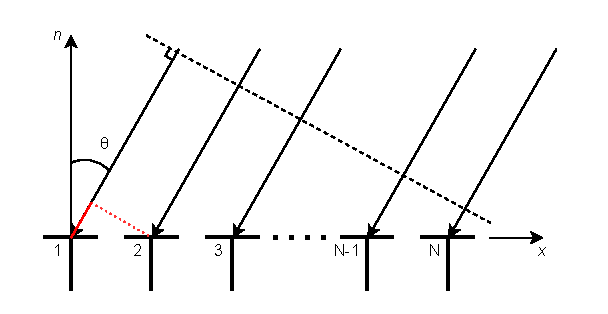
\includegraphics[width=0.8\textwidth,height=0.35\textheight,keepaspectratio]{antenna-array-interference}
    \caption{Приём сигнала на системе антенных элементов}%
    \label{fig:antenna-array-interference}
\end{figure}

Волновой фронт приходящего сигнала примем за плоский, т.к. цель находится в дальней зоне \cite{Chist2012}. 
Амплитуда напряжённости поля одинакова для всех элементов, однако фаза изменяется линейно в 
соответствии с направлением прихода сигналов. 
Примем расстояние от волнового фронта до 0-го элемента решётки за 0. 
Тогда для остальных элементов расстояние до фазового фронта может быть вычислено по формуле

\begin{equation*}
    d_n=x_n \cdot \sin\theta
\end{equation*}

\noindent здесь $x_n$ -- координата элемента в системе отсчёта с $0$ в начале антенной решётки и осью $Ox$ проведённой вдоль 
плоскости АР. $\theta$ -- угол между направлением прихода сигнала и нормалью к плоскости антенной решётки. 

Отсюда набег фазы для n-го элемента можно записать как 

\begin{equation*}
    \phi_n = k x_n \cdot \sin\theta
\end{equation*}

где $k=\frac{2\pi}{\lambda}=\frac{2\pi f}{c}$ -- волновое число. Здесь $\lambda$ -- длина волны, $f$ -- частота сигнала, $c$ -- скорость света.

Тогда сигнал, наведённый на n-ый элемент рассчитывается по формуле

\begin{equation}\label{eqn:antenna-array-element-value}
    E_n=A\cdot e^{j\cdot 2 \pi f x_n \frac{\sin{(\theta)}}{c}}
\end{equation}

Если объединить значения наведённого сигнала со всех элементов в одну последовательность, 
то получится сигнал комплексной синусоиды.

Период этого сигнала изменяется в зависимости от угла прихода, принимая значения от $0$ до $2\pi fx_n/с$.
Форма сигнала, принятого решёткой, зависит от количества целей. Данный сигнал является суммой частотно ограниченного множества сигналов. 

Зная природу сигнала и правильно выбрав точки для его измерения, можно уменьшить число измерений, 
дополнив снятый сигнал с помощью интерполяции.

В разделе \ref{sect:interpolation-modeling} проведено моделирование данного метода, 
описаны сложности разработки и исследования данного метода, приведены предполагаемые достоинства, 
недостатки и возможные пути развития.

